\subsection{\textit{Bussiness Aspects of Software Engineering}}
	
	Lelang merupakan salah satu metode pertukaran barang dan jasa dengan metode penetapan harga yang berbeda dengan perdagangan. Oleh karena itu, lelang juga termasuk dalam kategori bisnis. Yang menarik adalah, ketika bisnis digabungkan dengan teknologi atau yang sering disebut \textit{e-commerce}, hal yang sekedar pertukaran barang bertransformasi menjadi sebuah sistem interaktif yang kompleks dimana tujuan utamanya adalah menarik pengunjung/pengguna untuk menyelesaikan sebuah transaksi. Hal ini tentu sangat krusial, penting, dan tertantang untuk menyelesaikannya. \\
	\indent Dalam mencapai kesuksesan dan tingkat kompetitif yang tinggi, haruslah menyediakan layanan dengan kesan \textit{user experience (UX)} yang positif bagi para penggunanya. Morville  \cite[p.~27]{a-set-of-heuristics-2014} , dalam studi yang dilakukannya, menyebutkan bahwa UX tercakup dalam 6 aspek esensial, yaitu \begin{enumerate}[label=\alph*.]
		\item \textit{useful}
		\item \textit{usable}
		\item \textit{findable}
		\item \textit{desirable}
		\item \textit{accessible}
		\item \textit{credible}.
		\end{enumerate}
	
	\indent Hasil-hasil temuan penting yang menarik dalam pengaruh \textit{user experience}, adalah sebagai berikut dikutip dari sebuah sumber adalah sebagai berikut:
	\begin{enumerate}[label=\alph*.]
		\item \textit{User tend to leave if a page loads more than 3 seconds};
		\item \textit{79\% of users won't return if the web's performance and experience is poor}; \textit{and}
		\item \textit{44\% of users will tell the poor experiences to their friends}.
	\end{enumerate}
	
	\indent Selain dari faktor \textit{user experience} dan \textit{performance}, beberapa hal yang menjadi poin penting dan menarik dalam beberapa studi yang terkait adalah sebagai berikut:
	\begin{enumerate}[label=\alph*]
		\item \textit{Familiarity} - yang dapat didefinisikan sebagai tingkat familier atau kesamaan dengan sistem sejenis ternyata dapat membangun \textit{trust} sehingga mensugesti pengguna untuk menyelesaikan transaksi yang dilakukan;
		\item \textit{Usability} yang memudahkan pengguna dalam menyelesaikan transaksi; dan
		\item Aspek-aspek psikologi seperti pemilihan warna, penggunaan \textit{icon} yang sesuai, seperti \textit{icon} gembok pada halaman pembayaran ternyata dapat mengesankan \textit{security} pada pengguna.
	\end{enumerate}
	
	
	\begin{figure}[t]
		\centering
		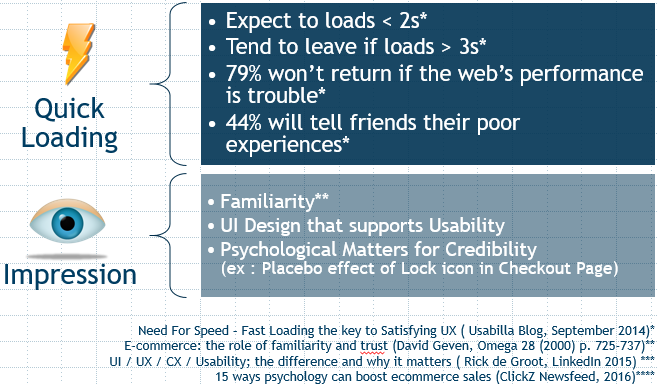
\includegraphics
		[width=\textwidth]
		{images/bab3/analisa/user-centered.png}
		\caption{Aspek Bisnis dalam \textit{Software Engineering}}
		\label{user-centered-analysis}
	\end{figure}
	
	\indent Dari hasil temuan ini, dapat disimpulkan bahwa \textit{user experiences, performances, usability} dan psikologi memiliki pengaruh besar dalam kesuksesan lelang \textit{online} dalam menarik hati para penggunanya. Hal ini akan mempengaruhi definisi kebutuhan fungsionalitas yang akan dibahas dalam Subbab \ref{keb-fungsional}.
		
		
		